\documentclass[12pt]{article}
\usepackage[utf8]{inputenc}
\usepackage[margin=1in]{geometry}
\usepackage{hyperref}
\usepackage[backend=bibtex]{biblatex}

\usepackage{indentfirst}
\usepackage{amsmath}
\usepackage{graphicx}
\usepackage{caption}
\usepackage{subcaption}


\bibliography{references} 

\graphicspath{ {images/} }

\renewcommand{\baselinestretch}{1.2}

\title{Discovering Panoramas in Web Videos}

\author{Lingfeng Huang \\ lhuang58@wisc.edu 
   \and Fang Wang \\ fwang64@wisc.edu}
  
\date{12/2016}


\begin{document}
\maketitle

\section*{Note}
Our website is available \href{http://lhuang58.github.io}{here. lhuang58.github.io}\\
Due to the file size of video test segments, we are not able to upload those to the Learn@UW. We send the video segments to you by email. The name of the video corresponds to the Figure number in this report.

\section*{Abstract and Problem Statement}
Panoramas have been widely used in may applications in multimedia, but the main constraint for panoramas is that they must be taken by people who physically present at the place. In this project, we implement our version of Discovering Panoramas in Web Videos by Liu et al.\cite{Liu}. Our goal is to solve two problems: First, the program should be able to select optimal segments within a given web videos to synthesis a panorama using visual quality measurement introduced in Liu et al.\cite{Liu} Second, the program should be able to generate a set of panoramas if multiple panoramas can be synthesised in a given video. 
The whole procedure is a optimization problem where we optimize the three criteria which are wide field of view, mosaicability, and high image quality.
\section{Introduction}
The emerge of the idea "Panorama" has to be dated back to early 20 A.D. and was a means of generating an 'panoptic' view of a vista\cite{wikipedia}. Nowadays, 
with the help of advancement of technology, people are able to create desired panorama by simply rotating their cell phones and clicking the shot button. The process of synthesizing panorama is relatively straight forward. First step is to take successive photos from the same optical center. The next step is finding the alignment between
each image and warping accordingly, and the final step is interpolating the warped image and applied certain blending to remove the visible seams. However, the problem with creating
panoramas using above approach is that people are required to physically appear at the place where they take the images, which means if people want to take a panorama of Time Square in New York, they have to fly over New York to do so. \par
Compared to a sequence of images, videos are still shot from the same optical center and cover a wide field-of-view although some segments within videos have relatively low image quality and there might also have moving objects. Liu et al.\cite{Liu}suggests an approach that synthesizing panoramas by identifying proper segments within videos as panorama source. They convert the problem into a optimization problem, and set up three constraints in order to evaluate the video segments.\cite{Liu} ei al. indicates that in order to be a appropriate panorama source, a video segment should cover a wide field-of-view based on the definition of panorama imagery,  be "mosaicable" and the frames should have high image quality\cite{Liu}.

\section{Visual Quality Measure}
We measure the visual quality of a single frame based on two terms, one is the incorrectness of the motion model $\mathit{E_{vm}(S_i)}$ and the other is the source image visual quality $\mathit{E_{vv}(S_i)}$. Then by setting up the visual quality distortion $\mathit{E_v(S_i)}$, we can obtain the visual quality measure.
\begin{equation}
\mathit{E_v(S_i)} = \alpha_m\mathit{E_{vm}(S_i)} + \alpha_v\mathit{E_{vv}(S_i)}
\end{equation}
By default, we set both weights $\alpha_v$ and $\alpha_m$ to be 1.0.
\subsection{Source Image Visual Quality}
The source image visual Quality $\mathit{E_{vv}(S_i)}$ is defined as how blurry and how blocky the image is. We use the idea from Tong et al.'s \cite{Tong} method of measuring blurring artifacts by using Haar Wavelet Transform. Tong et al. stated that by utilizing the ability of Haar Wavelet Transform, their method can be used not only on judging if an image is blurred or not, but also on determining the extent of blurriness of an image. Their method is discussed firmly in their paper and we will skip this part for now.
\begin{figure}[htbp]
	\begin{subfigure}[b]{0.49 \textwidth}
	\centering
	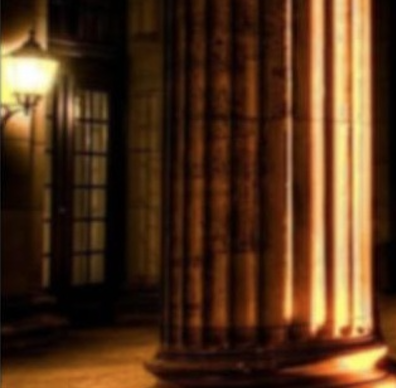
\includegraphics[width=7cm, height=7cm]{a}
	\caption{Blurriness: 0.8086}
	\label{default}
	\end{subfigure}
	%
	\hspace{1cm}
	%
	\begin{subfigure}[b]{0.49 \textwidth}
	\centering
	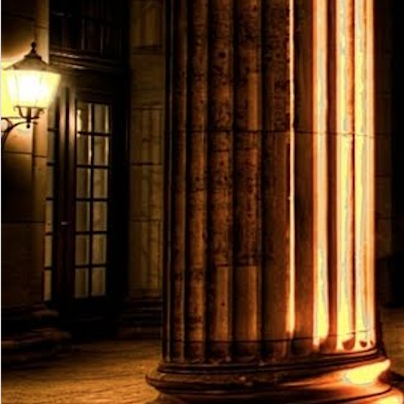
\includegraphics[width=7cm, height=7cm]{b}
	\caption{Blurriness: 0.3648}
	\label{default}
	\end{subfigure}
\caption{Blurriness measure compare}
\end{figure}
\par
The blockiness is measured by using the method of Wang et al., which estimates the average difference across block boundaries modulated by image activities \cite{Wang}. They came up with a computationally inexpensive and memory efficient feature extraction method to measure the blockiness which is ideal to our computational intensive procedures.
\begin{figure}[h]
	\begin{subfigure}[h]{0.49 \textwidth}
	\centering
	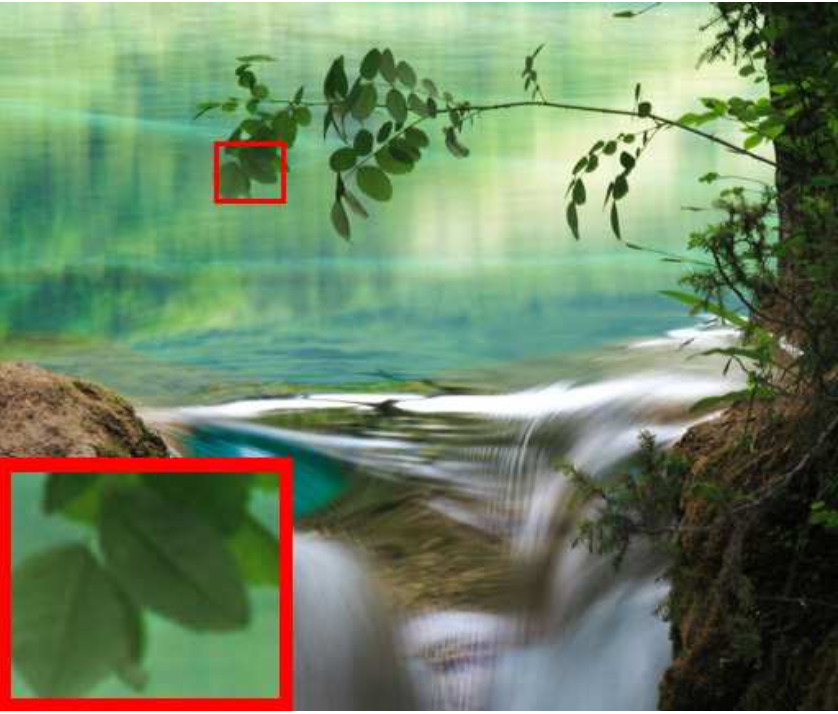
\includegraphics[width=7cm, height=7cm]{a1}
	\caption{Blockiness: 0.204}
	\label{default}
	\end{subfigure}
	%
	\hspace{1cm}
	%
	\begin{subfigure}[h]{0.49 \textwidth}
	\centering
	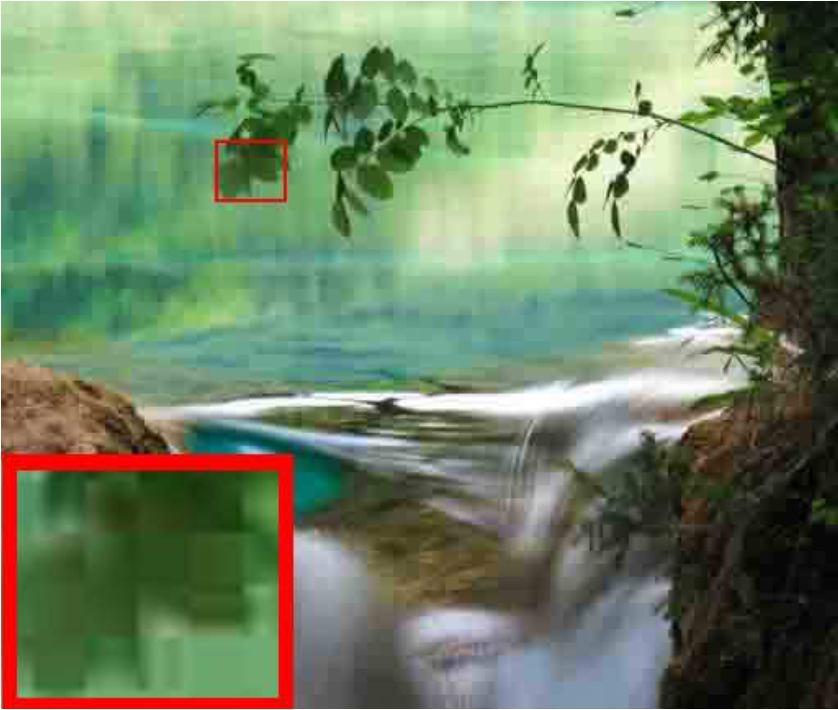
\includegraphics[width=7cm, height=7cm]{b1}
	\caption{Blockiness: 0.479}
	\label{default}
	\end{subfigure}
\caption{Blockiness measure compare}
\end{figure}

After obtain the blurriness and blockiness from all the frames within a given video segment, we can proceed to calculate the visual distortion for this segment as follows:
\begin{equation}
\mathit{E_{vv}(S_i)} = \sum_{\substack{\mathit{I_k\in S_i}}}\gamma \mathit{q_{bk}(I_k)} + (1 - \gamma)\mathit{q_{br}(I_k)}
\end{equation} 
where $\mathit{q_{bk}(I_k)}$ is the measurement of blockiness of given frame, and $\mathit{q_{br}(I_k)}$ is the measurement of blurriness. Weight $\gamma$ is set to 0.45 according to Liu et al. \cite{Liu}

\subsection{Incorrectness of Motion Model}
In order to achieve the "mosaicablity", we use a homography to model the motion between frames. By matching SIFT feature points, we are able to locate significant points between frames and thus obtain the homography. In practice, getting a high quality panorama from video requires the inter-frame motion is closed to its homography and few casual videos can achieve that. Therefore, we measure the error using the real motion vector from SIFT feature points and the predicted value by homography between two successive frames.
\begin{equation}
\mathit{E_{vm}(S_i)} = \sum_{\substack{\mathit{I_k\in S_i}}} \frac{1}{\mathit{n_k}} \sum_{\substack{\mathit{p_{j,k}}\in \mathit{S_i}}} \lVert \mathit{mv(p_{j,k})}, \mathit{mv_h(p_{j,k})} \rVert
\end{equation}
First, for each adjacent frame $\mathit{I_k}$ and $\mathit{I_{k + 1}}$ ,we find its matching SIFT feature pairs, then we calculate the homography using RANSAC based on these feature pairs. The notation $\mathit{mv(p_{j,k})}$ is the motion vector of $\mathit{j^{th}}$ SIFT feature point of frame $\mathit{I_k}$ and $\mathit{mv_h(p_{j,k})}$ is the predicted motion vector by homography at $\mathit{j^{th}}$ feature point. Then the error of $\mathit{j^{th}}$ feature point is taking the L1 norm of these two terms. Then we average the errors of all feature pair in each frame and obtain the incorrectness of motion model by summing up all the average. 
 
 \section{Extent of Scene}
 	The extent of scene $\varepsilon(\mathit{S_i})$ is defined as the scene covered by the video segment. Although it could be better if we maximizing the covering area to obtain a larger field of view, larger field of view often leads to more distortion. Hence, we decide to choose the reference frame where the distortion is minimum, in other words, we want the minimum area covered by segment $\mathit{S_i}$
	
\begin{figure}[h]
	\centering
	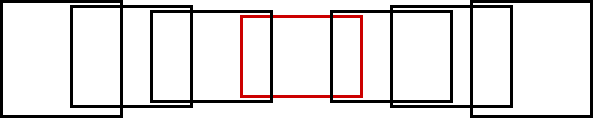
\includegraphics[width=15cm]{reference}
	\caption{All the other frames in the video are alignment to the reference frame, and we want to find the optimal reference frame so that the area covered by aligning all the frames to be minimized}
\end{figure}

In order to find the optimal reference frame, we search for all possible combination of panorama alignment as follows:
\begin{equation}
\mathit{r} = \mathrm{arg} \min_{\mathit{f_r} \in \mathit{S_i}} \bigcup_{\mathit{f} \in \mathit{S_i}} \mathit{I(f, f_r)}
\end{equation}
Then the extent of scene is defined as:
\begin{equation}
\varepsilon(\mathit{S_i}) = \bigcup_{\mathit{f} \in \mathit{S_i}} \mathit{I(f, r)}
\end{equation}
Liu et al. \cite{Liu} used generic polygon clipping for finding the minimum area covered. However, due to the complexity of their method, we chose another simplified approach. Although in this approach the accuracy declines, the complexity is reduced a decent amount. The simplified version of finding extent of a scene is done by finding the distance between the center of reference frame to all other frames:
\begin{equation}
\frac{1}{\mathit{n}} \sum_{\mathit{f \in S_i}}  \lVert \mathit{C_r}, \mathit{C_f} \rVert
\end{equation}
Where $\mathit{n}$ is the number of frames within the segment, $\mathit{C_r}$ is the center pixel of the reference frame and $\mathit{f_r}$ is the center pixel in a given frame.
\begin{figure}[h]
	\centering
		\begin{subfigure}{1\textwidth}
		\centering
			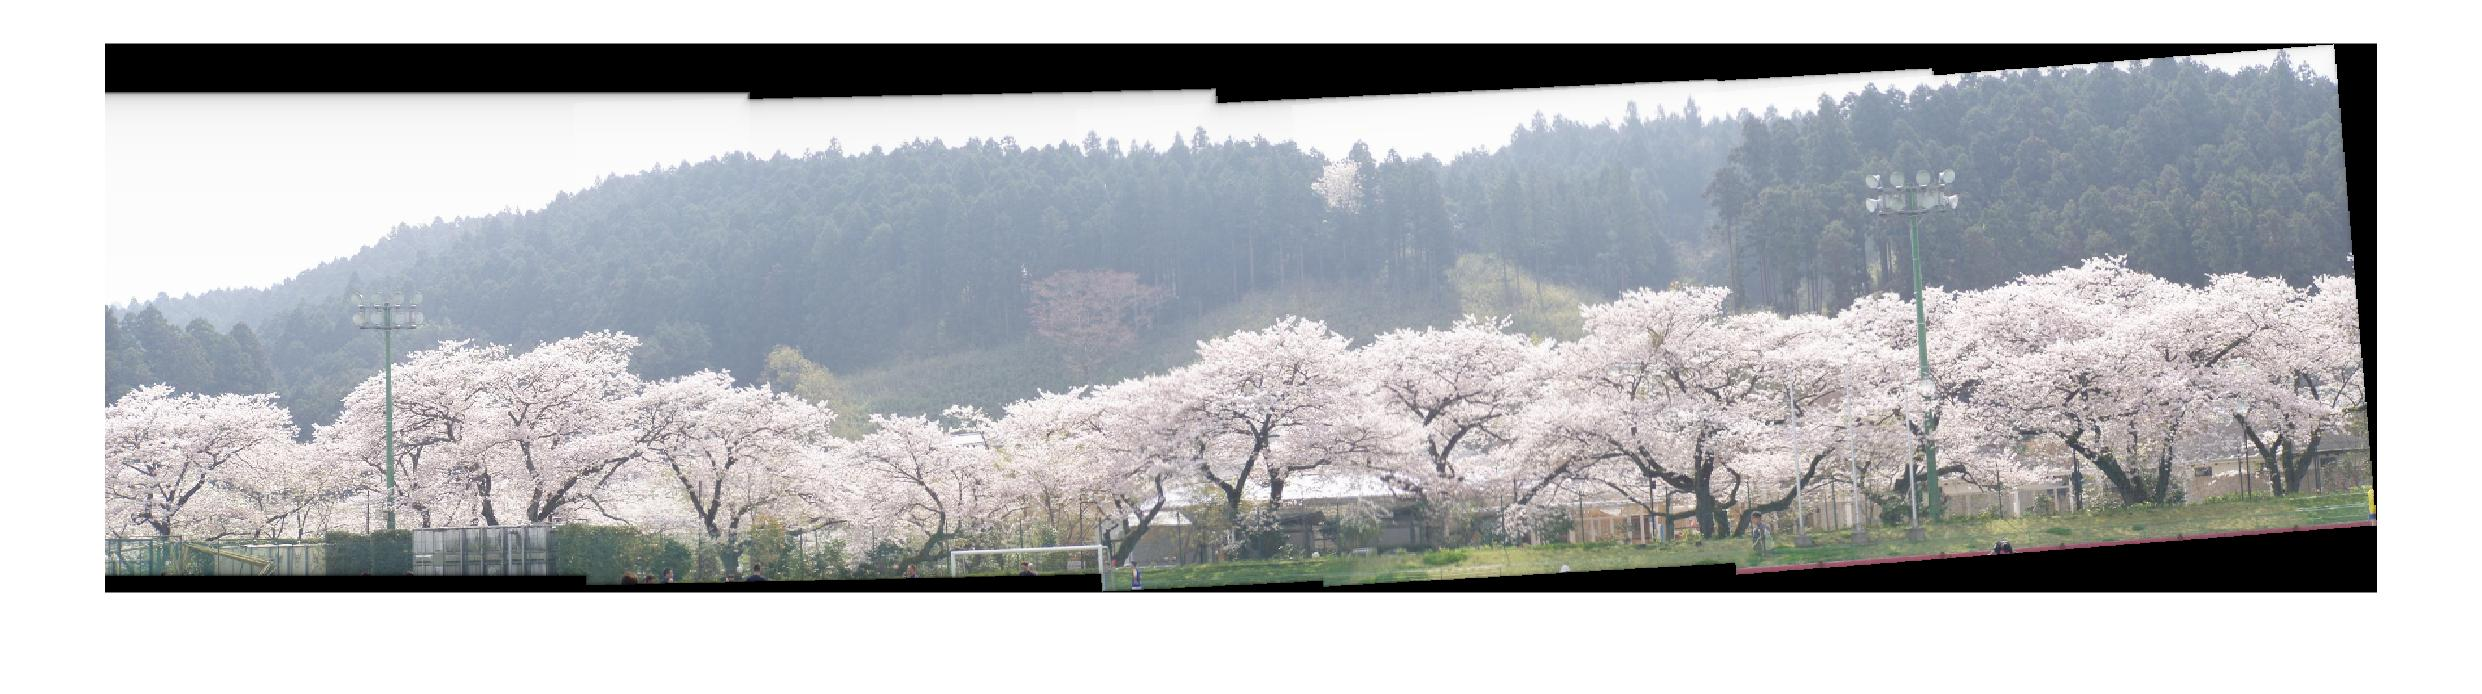
\includegraphics[height=3.5cm, width=15cm]{ref1}
			\caption{The reference frame is set at the left most frame}
			\label{fig:ref1}
		\end{subfigure}
		~
		\begin{subfigure}{1\textwidth}
		\centering
			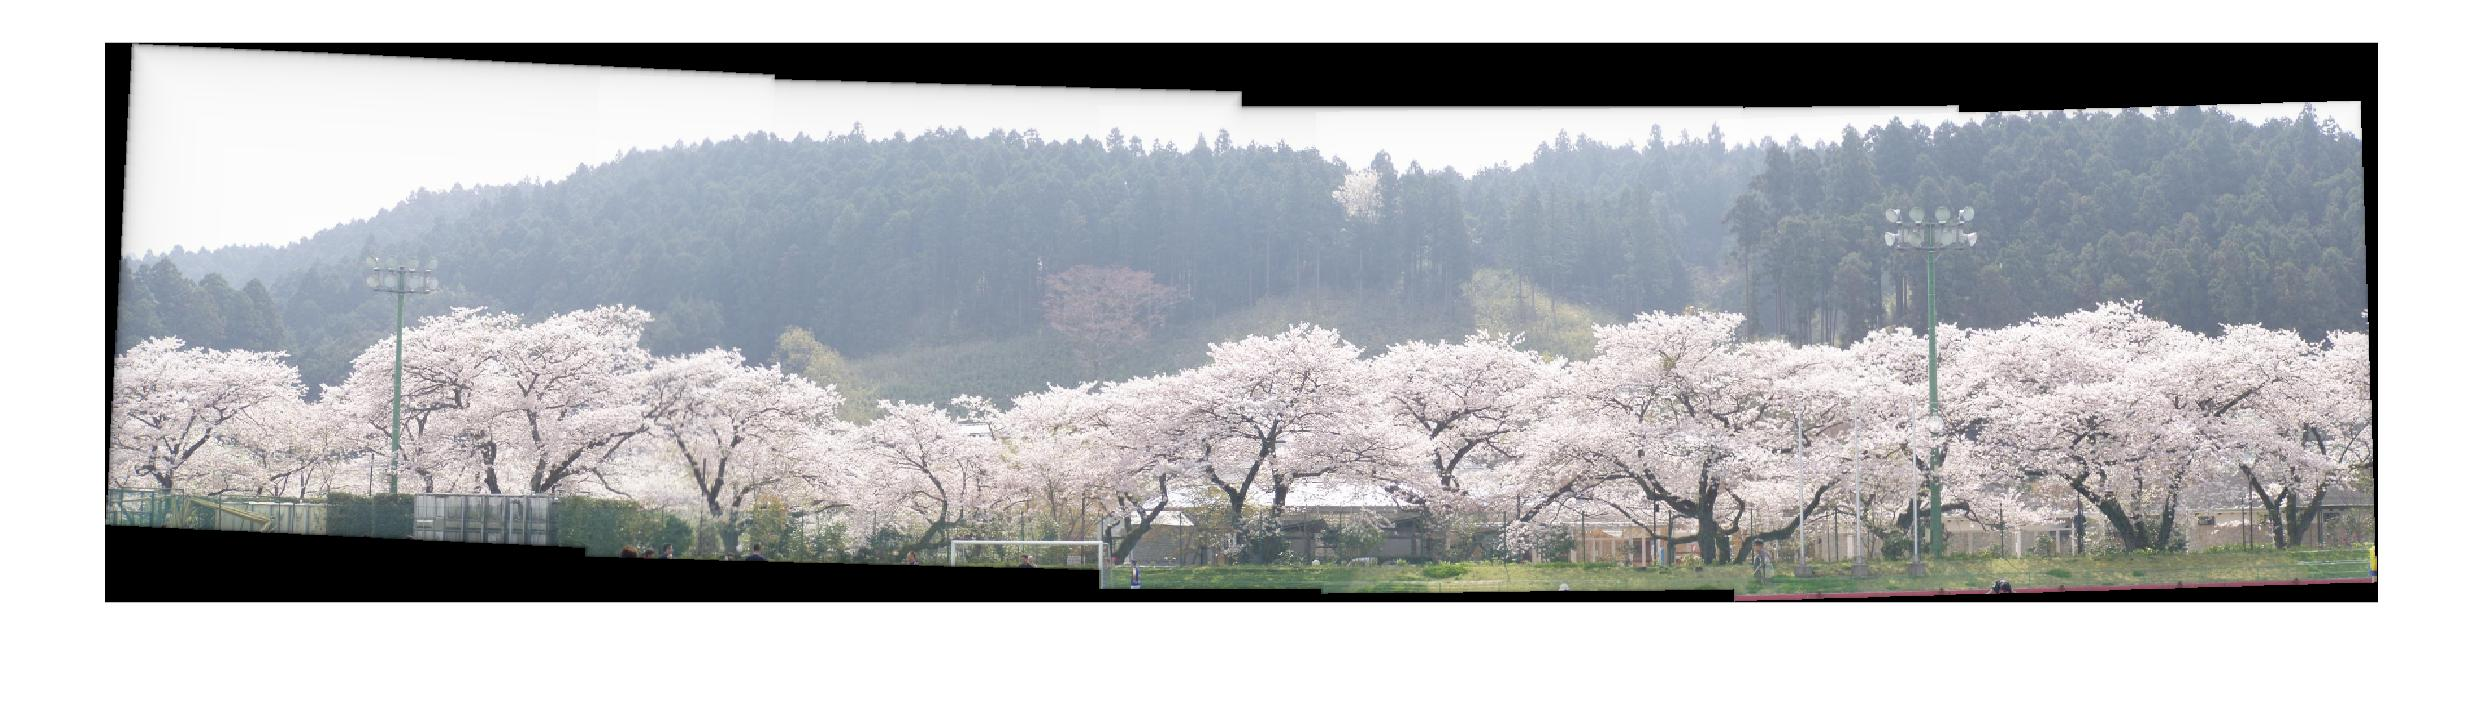
\includegraphics[height=3.5cm, width=15cm]{ref3}
			\caption{The reference frame is set at the center frame}
			\label{fig:ref3}
		\end{subfigure}
		~
				\begin{subfigure}{1\textwidth}
		\centering
			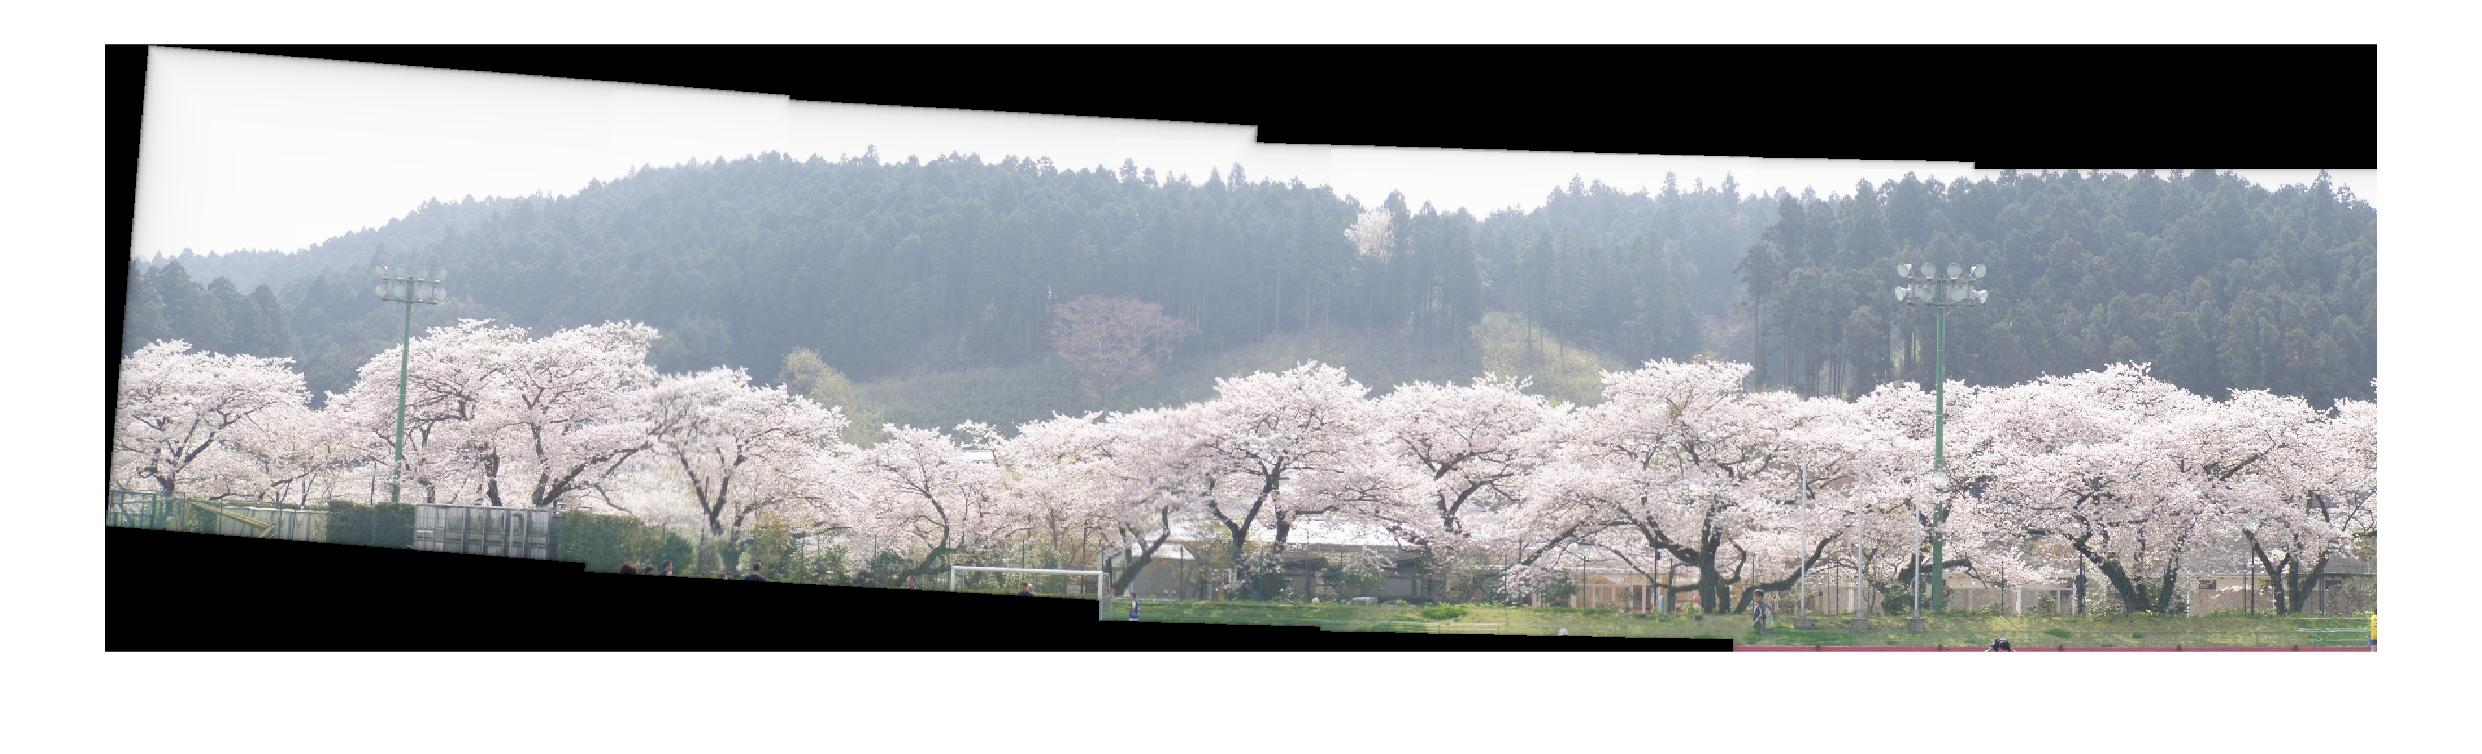
\includegraphics[height=3.5cm, width=15cm]{ref5}
			\caption{The reference frame is set at the right most frame}
			\label{fig:ref5}
		\end{subfigure}
		\caption{Difference reference frame results in different look of panorama}
\end{figure}
Figure 4 demonstrates when reference frame is the most left frame (the first frame in the image sequence), the middle frame and the right most frame. However, due to the relatively small distortion since this image sequence only has 5 images, the visual difference between three panoramas is subtle. 

\section{Experiments and Results for Determining a Panorama}
We randomly select some videos from Youtube and manually cut the video into several segments. Liu et al.\cite{Liu} use histogram based shot boundary detection to divide the video, while we use another approach which we describe in the next section. In order to test the correctness of the three panorama synthesis criteria, we choose to feed our algorithm with preprocessed video segments.\\
\\
\begin{figure}[h]
	\centering
	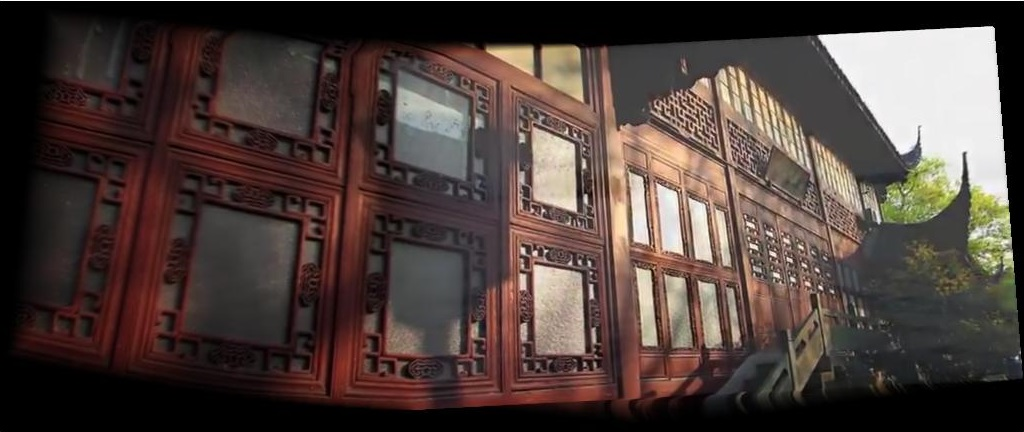
\includegraphics[width=9.5cm, height=3cm]{building562-691}
	\caption{Stitched using a video segment of a wood house}
\end{figure}\\
In figure 5, the motion error of the video estimated by our program is 598 (rounded to nearest integer) and since this segment has over 130 frames, so on average each frame has 4.6 error which is considered a good score in our standard. The image quality error for this segment is 23 which is also a relatively good score for a 640*360 (360p for short) resolution video. Therefore, we obtained a decent panorama from this segment.
\begin{figure}[h]
	\centering
	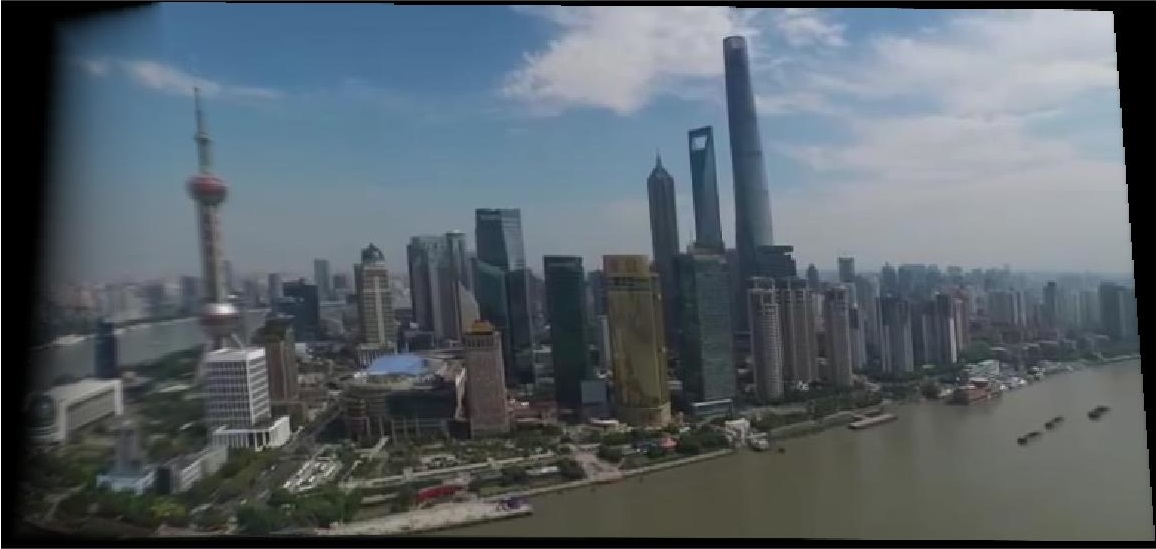
\includegraphics[width=9.5cm, height=3cm]{shanghai1309-1440}
	\caption{Stitched using a video segment of Shanghai city view taken by a drone}
\end{figure}
Figure 6 shows a shot from Shanghai, and the computed motion error is 587. Because the drone is very stable in the original video, the motion error is also what we expected. We also discovered that the image quality error of 360p videos from Youtube usually ranges from 20 to 45. Therefore, the panorama synthesized is also in good quality with only a subtle distortion. 
\begin{figure}[h]
	\centering
	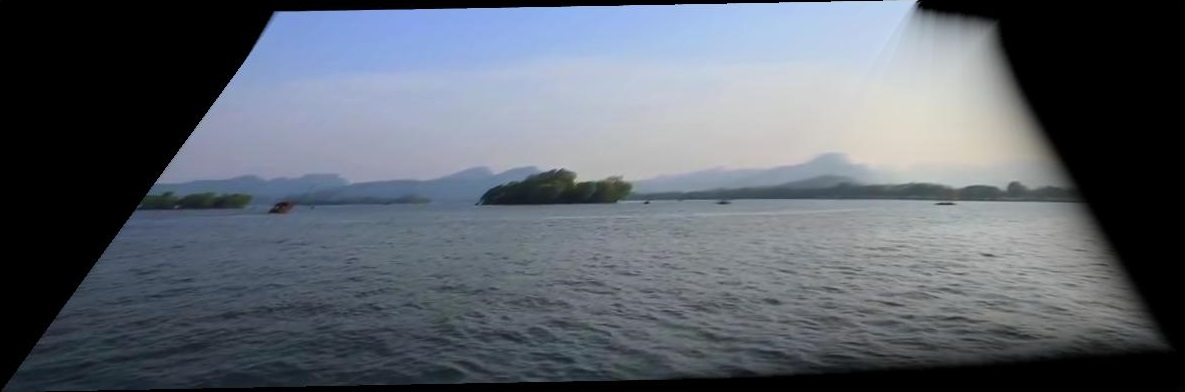
\includegraphics[width=9.5cm, height=3cm]{lakeError1206-1310}
	\caption{Stitched using a video segment of West Lake}
\end{figure}\\
Figure 7 shows a failure case. In the segment, we observed a large amount of object motion which is from the waves and the boats on the lake between frame to frame. As a result, the motion error for this segment is 1521. As a conclusion, our implementation of judging a segment works as expected and is able to distinguish between segments with different quality.

\section{Video Segment Fetching}
Liu et al.\cite{Liu} pre-process the given video by applying histogram based method for shot boundary detection and shot boundary is detected whenever the histogram intersection between two adjacent frames is below a threshold. 
However, we detect scene boundary by using the visual quality distortion.The idea is that in order to calculate the homography between two adjacent frames, we should have at least 4 SIFT matching pairs. According to our experiments, the video segments we have do not always have enough pairs to calculate homography when two frames are at scene boundary and even when they have enough pairs to calculate the visual quality error tend to be high. Thus, to solve the second problem, which is the program should be able to separate video segments to make a set of panoramas, we cut the whole video into segments with 20 frames each (since frame per second of a video is usually between 23 to 30, 20 frames segment roughly represents one second in the video which is neither too long nor too short), then we compute visual quality error for each segments. During the visual quality computation, there are two cases that clearly indicate a transition occurs in a given segment. One is that the transition frame is too sharp to have more than 4 SIFT matching pairs to the last frame. In this case, by setting the visual quality error to a large positive number (infinity in our case) we prevent the program from crashing due to not having enough matching pairs to calculate homography. Furthermore, since the larger the visual quality error is, the most likely it is a transition segment, setting the transition to infinity is acceptable. Another case is that when the transition occurs "smoothly", we need to set a threshold to separate segments. By examining the visual quality error of Figure 5 to 7, we decided to set the threshold to be 250. If any segment has visual quality error larger than 250, then it is likely to be a transition segment. In the final step of going through all segments to generate panoramas, we specify that there should be at least 3 consecutive segments to synthesis a valid panorama because a two second video is usually not having enough information (usually narrow in view). Since there may have several transition segments, we are able to generate several panoramas using the threshold of visual quality error as the signal of ending current panorama.

\section{Experiments and Results for fetching multiple Panoramas}
We define the types of videos that we might encounter while fetching as follows: \\
Case 1: A scene that is not capable of synthesizing panorama (a bad scene) followed by a scene that is a proper source for panorama (good scene) or vise versa. In both cases the program should only obtain one panorama from the good scene:
\begin{figure}[h]
	\centering
	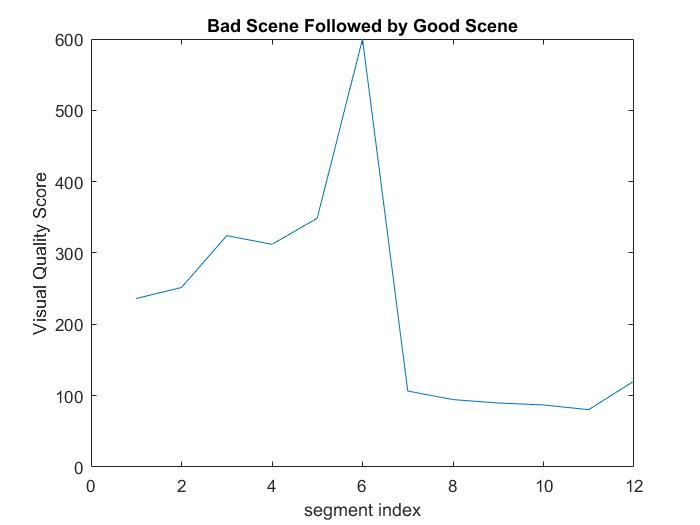
\includegraphics[width=10cm]{bad-good-fig}
	\caption{Visual quality error for Case 1}
\end{figure}\\
Above figure shows that the overall visual quality error for bad scene segments are high (over 250) and we have this sudden increase in the error at segment 6, thus we can say segment 6 has a high possibility of containing a scene transition. Thus, we want to drop all the segments before segment 7 due to high error. Then synthesizing the panorama use only segment 7 to 12.\\
Case 2: A good scene followed by a good scene. In this situation, the program should generate two panoramas :
\begin{figure}[h]
	\centering
	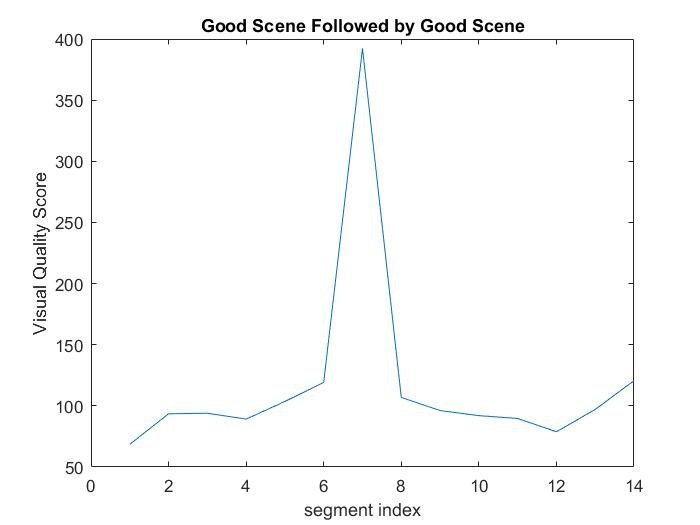
\includegraphics[width=10cm]{good-good-fig}
	\caption{Visual quality error for Case 2}
\end{figure}\\

It can be observed that before and after segment 7 there are two smooth segments series and a sudden increase in visual quality error at segment 7. In this case, we drop segment 7 and synthesize two panoramas from segment 1 to 5 and segment 7 to the rest segments.\\
Case 3: A bad scene followed by a bad scene. In this situation, we drop both scenes, and we can expect the overall visual quality errors are relatively high across all the segments.

\section{Conclusion and Limitations}
The result of this experiment is positive, we are able to solve the two problems which are determining a panorama and synthesis multiple panoramas. We learned a lot by reading the paper and searched for related domain knowledges. Since our experiment consists of several technique parts and we choose to implement in a simpler way, there are still limitations that need to be solved. For example, the whole process is significantly time-consuming. Because we are computing the visual quality score in each segments due to our segmentation algorithm, the complexity tends to be very high. During our experiments, a 250 frames video will take roughly 40 seconds to process. Another limitation is that because we are dropping the whole 20 frames segment with scene transition the field of view of the final panoramas are reduced in small amount but the effect is subtle if the the panorama is made by a longer video segment. 

\section{Overview of our project}
Credit to: part of the synthesis and blending stage of panorama synthesis is from project 4 CS534. TODO: blurness and blockiness credit if necessary\\
Number of lines: TODO: 400lines?\\
Contribution: 
Lingfeng Huang: establish the skeleton of the program and the report, mainly focus on solving the first problem which is determine a panorama. 
Fang Wang: focus on solving the second problem which is how to separate different panoramas. Suggested several algorithms to implement and speed up the code when working with Lingfeng to solve the first problem. Revised and reformed the report.

\iffalse
this part is comment and you can delete this part later. I attached the requirements of Dyer and you can check if there is any part we can enhance.
FROM cs534 homepage: At the beginning of your report give the title, team members, link to your project's web page if you have one (a web page is optional and will count as extra credit points for the course), and an abstract of your project. Your report should describe the problem, the approach implemented, a summary of experiments, and evaluation of results. The length will depend a lot on the type of project. Most reports will be about 10-15 pages long. The style should be in the form of a conference paper. That is, title, abstract, introduction, motivation, problem statement, related work, theory, method, experimental results, concluding remarks, and references. Include at the end of your report a description of what code you got from elsewhere that you did not write, and what code your team wrote; include approximate number of lines of code written. Also describe what the main contributions were of each team member.
\fi

\newpage
\printbibliography

\end{document}